\documentclass{article}

\usepackage{subfig}
\usepackage{tikz}

\usepackage{amsmath}
\usepackage{listings}
\usepackage{algorithm}
\usepackage[noend]{algpseudocode} %for pseudo code, include algorithmicsx automatically

% for better Haskell code outlook
%% \lstdefinelanguage{Haskell}{
%%   basicstyle=\small\ttfamily,
%%   flexiblecolumns=false,
%%   basewidth={0.5em,0.45em},
%%   literate={+}{{$+$}}1 {/}{{$/$}}1 {*}{{$*$}}1 {=}{{$=$}}1
%%            {>}{{$>$}}1 {<}{{$<$}}1 {\\}{{$\lambda$}}1
%%            {\\\\}{{\char`\\\char`\\}}1
%%            {->}{{$\rightarrow$}}2 {>=}{{$\geq$}}2 {<-}{{$\leftarrow$}}2
%%            {<=}{{$\leq$}}2 {=>}{{$\Rightarrow$}}2
%%            {\ .}{{$\circ$}}2 {\ .\ }{{$\circ$}}2
%%            {>>}{{>>}}2 {>>=}{{>>=}}2
%%            {|}{{$\mid$}}1
%% }[keywords,comments,strings]

\lstloadlanguages{C, Haskell, Python}

\lstset{
  showstringspaces = false
}

\begin{document}

\title{The longest palindrome}
\author{Larry LIU Xinyu}
\maketitle

\section{The problem}
Palindrome is a symmetric sequence of elements. It doesn't change when gets reversed.
For example, the English word `madam' is a palindrome. If $S$ is a palindrome, we have
$S = reverse(S)$. Palindrome can be a number, a string, a piece of DNA genome,
or even music. A palindromic sub-string part of the string that is a palindrome.
For example `issi' is a palindromic sub-string in word `Mississippi'. There can be
multiple palindromic sub-strings. The problem is to find the longest palindromic
sub-string. Given `Mississippi` for example, the longest plindromic sub-string is
`ississi'.

\section{Manacher's algorithm}

There are several methods to solve this problem. The brute-force solution is to
enumerate all the sub-strings, filter the palindromic ones, and pick the longest.
There are $n(n+1)/2$ sub-strings where $n$ is the length of the string (Empty
string is ignored). Thus the performance is quadratic.

Another method is to use suffix tree. If $w$ is a palindromic sub-string of
$S$, then it must be sub-string of $reverse(S)$ also.
For example, ``issi'' is a palindromic sub-string of ``Mississippi''.
and its reversed form ``ippississiM''.

Based on this fact, we can find the longest palindrome by
searching the longest common sub-string for $S$ and $reverse(S)$.

\begin{equation}
LCS(T_{\textrm{suffix}}(S + reverse(S)))
\end{equation}

Function $LCS$ finds the
longest common sub-string in the suffix tree in linear time.

The key point is to construct the suffix tree efficiently. There are
some good algorithms achieves linear time performace, like Ukkonen's algorithm\cite{Ukkonen95}.
Generalised suffix tree can find the longest palindromic sub-string in linear time.

Suffix array provides a easier solution than suffix tree. But it downgrades
the performance to $O(n \lg n)$.

We'll explain a linear time algorithm found by Glenn K. Manacher in 1975 \cite{Manacher75}.
This method scan the string and reuse the information gained during the scan.

For given string $S = \{s_1, s_2, ..., s_n\}$, let $P = \{p_1, p_2, ... p_n\}$ be a table.
$p_i$ is defined as the following.

\begin{equation}
p_i = max \{ d | \{s_{i-d}, ..., s_{i+d}\} \textrm{\ is palindrome}, d = 1, 2, 3, ...\}
\label{eq:p-table}
\end{equation}

We call $P$ the palindrome table.
$p_i$ tells us how long we can extend from the $i$-th element in $S$ to
left and right to form a palindrome. In other words the sub-string
$\{s_{i-p_i}, s_{i-p_i+1}, ..., s_i, ..., s_{i+p_i}\}$ is the longest palindromic sub-string
at the center of $i$. We donote this sub-string as $S_{(i, p_i)}$.
Below table shows an example for string `eneven'.

%\begin{table}
\begin{tabular}{|c|c|c|c|c|c|c|}
\hline
$S$ & e & n & e & v & e & n \\
\hline
$P$ & 1 & 2 & 1 & 3 & 1 & 1 \\
\hline
$S_{(i, p_i)}$ & e & ene & e & neven & e & n \\
\hline
\end{tabular}
%\end{table}

The first value $p_1 = 1$, the palindrome at the center of the first element contains
only one character ``e''. The second value $p_2 = 2$, it means we can extend from
the second element 2 characters to both sides. It gives the
palindrome ``ene''. The fourth value $p_4 = 3$, we can extend 3 characters to get
the palindrome ``neven''. We can think
$p_i$ as the `radius' of the palindrome at center $i$.

However, there is a problem in the definition of $p_i$. In equation (\ref{eq:p-table}),
the length of the palindrome is forced to be odd number. It doesn't work
for even length. For example, the $P$ table for string $S = ...issi...$ is below.

\begin{tabular}{|c|c|c|c|c|c|c|}
\hline
$S$ & ... & i & s & s & i & ... \\
\hline
$P$ & ... & 1 & 1 & 1 & 1 & ... \\
\hline
\end{tabular}

Acutally, we need it to be something like below.

\begin{tabular}{|c|c|c|c|c|c|c|c|}
\hline
$S$ & ... & i & s &   & s & i & ... \\
\hline
$P$ & ... &   &   & 2 &   &   & ... \\
\hline
\end{tabular}

One solution is to insert a special delimiter $\# \notin S$ between all elements in $S$ to
turn it into another string $S'$.

\begin{equation}
S' = \{\#, s_1, \#, s_2, \#, ..., \#, s_n, \#\}
\end{equation}

There are two cases.

\begin{itemize}
\item For the odd length palindrome, Let the length be $L = 2k + 1$.

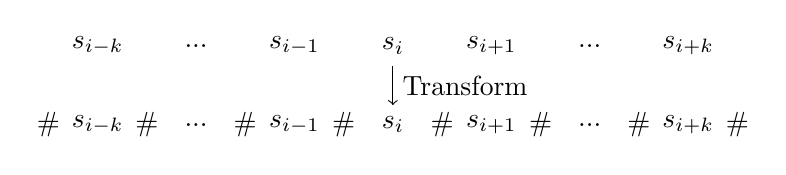
\begin{tikzpicture}[scale=2.5]
  \draw (-1.5cm, .4) node{$s_{i-k}$};
  \draw (-1cm, .4) node{...};
  \draw (-0.5cm, .4) node{$s_{i-1}$};
  \draw (0, .4) node{$s_i$};
  \draw (0.5cm, .4) node{$s_{i+1}$};
  \draw (1cm, .4) node{...};
  \draw (1.5cm, .4) node{$s_{i+k}$};

  \foreach \x in {-1.75, -1.25, ..., 1.75} {
    \draw (\x cm, 0) node{\#};
  }

  \draw (-1.5cm, 0) node{$s_{i-k}$};
  \draw (-1cm, 0) node{...};
  \draw (-0.5cm, 0) node{$s_{i-1}$};
  \draw (0, 0) node{$s_i$};
  \draw (0.5cm, 0) node{$s_{i+1}$};
  \draw (1cm, 0) node{...};
  \draw (1.5cm, 0) node{$s_{i+k}$};

  \draw[->] (0, .3) -- (0, .2) node[right]{Transform} -- (0, .1);

\end{tikzpicture}

After the transformation, the center of the new palindrome is still $s_i$. In the
new palindrome talbe $P'$, the value correspond to $s_i$ is $p'_j = 2k + 2$.

\item For the even length palindrome, Let the length be $L = 2k$.

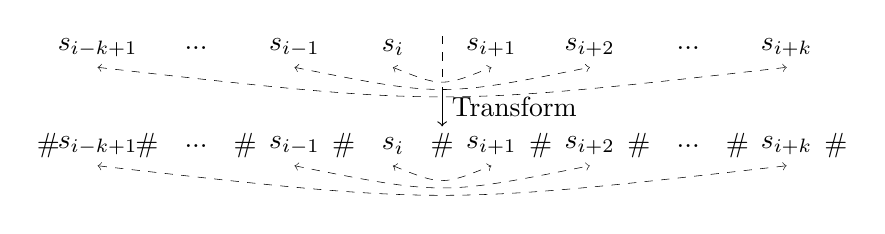
\begin{tikzpicture}[scale=2.5]
  \draw (-1.75cm, .5) node{$s_{i-k+1}$};
  \draw (-1.25cm, .5) node{...};
  \draw (-0.75cm, .5) node{$s_{i-1}$};
  \draw (-0.25cm, .5) node{$s_i$};
  \draw (.25cm, .5) node{$s_{i+1}$};
  \draw (0.75cm, .5) node{$s_{i+2}$};
  \draw (1.25cm, .5) node{...};
  \draw (1.75cm, .5) node{$s_{i+k}$};

  \draw[dashed, very thin] (0, .35) -- (0, .6);
  \foreach \x/\y in {0.25/0.3, 0.75/0.25, 1.75/0.2} {
    \draw[dashed, very thin, <->] (-\x cm, .4) .. controls (0, \y) .. (\x cm, .4);
  }

  \foreach \x in {-2, -1.5, ..., 2} {
    \draw (\x cm, 0) node{\#};
  }

  \draw (-1.75cm, .0) node{$s_{i-k+1}$};
  \draw (-1.25cm, .0) node{...};
  \draw (-0.75cm, .0) node{$s_{i-1}$};
  \draw (-0.25cm, .0) node{$s_i$};
  \draw (.25cm, .0) node{$s_{i+1}$};
  \draw (0.75cm, .0) node{$s_{i+2}$};
  \draw (1.25cm, .0) node{...};
  \draw (1.75cm, .0) node{$s_{i+k}$};

  \foreach \x/\y in {0.25/-0.2, 0.75/-0.25, 1.75/-0.3} {
    \draw[dashed, very thin, <->] (-\x cm, -0.1) .. controls (0, \y) .. (\x cm, -0.1);
  }

  \draw[->] (0, .3) -- (0, .2) node[right]{Transform} -- (0, .1);

\end{tikzpicture}

After the transformation, the center of the new palindrome becomes a delimiter \#. In the
new palindrome talbe $P'$, the value correspond to the new center is $p'_j = 2k + 1$.
\end{itemize}

In both cases, we have the relationship $L = p'_j - 1$. If we construct a palindrome
table for the transformed string, each value in the table that not for the delimiter
is 1 unit longer than the length of the original palindromic sub-string in $S$.
Because the the maximum value in the palindrome table is bound to the longest
palindromic sub-string, the longest palindrome problem can be solved with the following
strategy.

\begin{enumerate}
\item Transform to a new string with speical delimiter;
\item Construct the palindrome table effeciently;
\item The longest palindromic sub-string can be located by finding the maximum value
in the palindrome table. Its length can be given by decreasing the maximum value by one.
\end{enumerate}

\section{The brute-force scan}
The brute-force method scans the transformed string from left to right. For each position
$i$, it checks if $s_{i+k} = s_{i-k}$ for $k = 0, 1, 2, ...$ can be satisfied.

\begin{algorithmic}[1]
\Function{Palindrome}{$S$}
  \State $S' \gets $ empty
  \For{$i \gets 1$ to $|S|$}
    \State $S' \gets S' + \{\#, s_i\}$
  \EndFor
  \State $S' \gets S' + \{\#\}$
  \State $P \gets \{0, 0, ..., 0\}$ \Comment{length of $|S'|$}
  \For{$i \gets 1$ to $|S'|$}
    \For{$k \gets 0, 1, 2, ...$}
      \If{$1 \leq i \pm k \leq |S'|$ and $s'_{i-k} = s'_{i+k}$}
        \State $p_i \gets p_i + 1$
      \Else
        \State break
      \EndIf
    \EndFor
  \EndFor
  \State \Return $max\{p_i\} - 1$
\EndFunction
\end{algorithmic}

The worst case happens when all the characters are same, for instance ``aaa...a'', that
there are $n$ same characters `a'. The brute-force method is quadratic ($O(n^2)$).

\section{Manacher's method}
The key to Manacher's method is information reusing. In order to construct
the palindrome table $P$ effeciently, we need {\em reuse} so far gained result
$p_1 \sim p_{i-1}$ when caculate $p_i$.

Observe the brute-force solution. It compares $s_{i+1}$ with $s_{i-1}$, and
$s_{i+2}$ with $s_{i-2}$, ... The element to the right of $s_i$,
may have been examined and it may belong to some previously found palindromic
sub-string. In other words there may be some $j \in [1 \sim i-1]$ that satisfies
$i \leq j + p_j$. This is illustrate in figure \ref{fig:right-most}. We can record the right most position that a palindromic
sub-strings can rich:

\begin{equation}
r_m = max \{ j + p_j, j < i\}
\end{equation}

\begin{figure}[htdp]
\centering
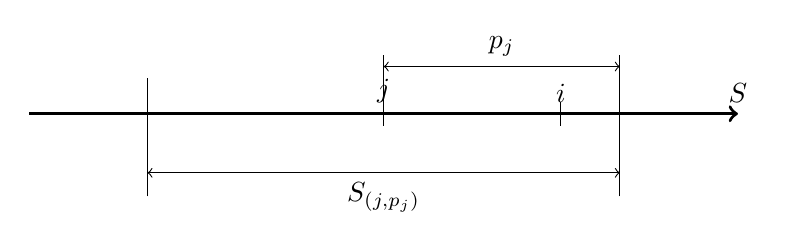
\begin{tikzpicture}[scale=1.5]
  \draw[->, very thick] (-3, .5) -- (0, .5) node[above]{$j$} -- (1.5, .5) node[above]{$i$} -- (3, .5) node[above]{$S$};
  \draw[<->] (-2, 0) -- (0, 0) node[below]{$S_{(j, p_j)}$} -- (2, 0);
  \draw[thin] (-2, -0.2) -- +(0, 1);
  \draw[thin] (2, -0.2) -- + (0, 1.2);
  \draw[thin] (0, 0.4) -- + (0, 0.6);
  \draw[thin, <->] (0, .9) -- +(1, 0) node[above]{$p_j$} -- ++ (2, 0);
  \draw[thin] (1.5, 0.4) -- + (0, 0.2);
\end{tikzpicture}
\caption{Element at $i$ belongs to palindrome $S_{(j, p_j)}$. The palindrome extends to the right of $i$.}
\label{fig:right-most}
\end{figure}

When scan to the $i$-th position from left to right, we compare $i$ with $r_m$ first to see if this position
has been examined before, so that we can reuse the $p_1 \sim p_{i-1}$ information. There are two cases:

\subsection*{Case 1, $i > r_m$}

Because $i > max \{j+p_j, j < i \}$, $s_i$ doesn't belongs to any known palindrome. What we can do is as
same as the brute-force method, scan and compare the symmetric elements $s_{i+k}$ and $s_{i-k}$ until we
find an unmatch. The farest $k$ is the value of $p_i$.

\begin{algorithmic}[1]
\If{$i > r_m$}
  \State $p_i \gets 1$
  \While{$s_{i+p_i} = s_{i-p_i}$}
    \State $p_i \gets p_i + 1$
  \EndWhile
\EndIf
\end{algorithmic}


\subsection*{Case 2, $i \leq r_m$}

Because $i \leq max \{j + p_j, j < i\}$, $s_i$ belongs to some known palindrome. There are three sub-cases:

\subsubsection*{Sub-case 1}

As shown in figure \ref{fig:subcase1}, Denote the $j$ leads to $r_m$ as $j_m$. The palindrome at the
center of $j_m$ is $A = S_{(j_m, p_{j_m})}$. The two elements out of the bound of $A$ are different.
They are represented as $x$ and $y$, $x \neq y$. Because element at $i$ belongs to the palindrome
at the center of $j_m$, its symmetric position to $j_m$ is $2j_m - i$. This is because
$\frac{i + (2j_m -i)}{2} = j_m$. Denote the palindrome at the center of this position as $B$.
In sub-case 1, the left bound of $B$ is to the left of $A$.

\[
left(B) < left(A)
\]

This tells us that $x \in B$. According to the definition of palindrome, there must be a symmetric
element $x'$ in $B$, that $x' = x$. Because $x' \in A$, again, there must be a symmetric element
$x''$ in palindrome $A$, so that $x'' = x$. Since $x \neq y$, we have $x'' \neq y$, this means that
the `radius' of the palindrome at the center of $i$ is equal to the distance between points $a$ and $b$.

\[
r = |a - b| = j_m + p_{j_m} - i
\]


\begin{figure}[htdp]
\centering
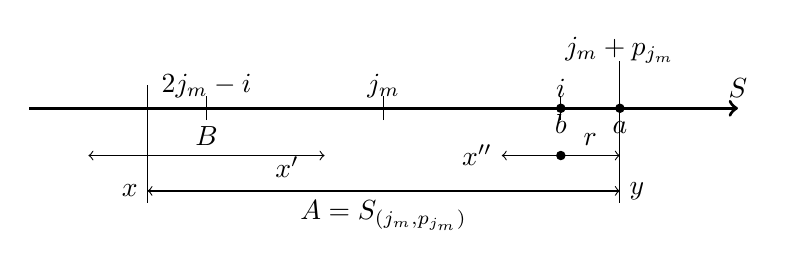
\begin{tikzpicture}[scale=1.5]
  \draw[->, very thick] (-3, .5) --(-1.5, .5) node[above]{$2j_m - i$} --
         (0, .5) node[above]{$j_m$} -- (1.5, .5) node[above]{$i$} --
         (3, .5) node[above]{$S$};
  \draw[thin] (1.5, 0.4) -- + (0, .2); %tick for i
  \draw[thin] (-1.5, 0.4) -- + (0, .2); %tick for 2j_m - i
  \draw[thin] (0, 0.4) -- + (0, .2); %tick for j_m

  % label a, b
  \draw (1.5, .2) node[above]{$b$} (2, .2) node[above]{$a$}
        (2, .8) node[above]{$j_m + p_{j_m}$};
  \filldraw (1.5, .5) circle [radius=1pt]
            (2, .5) circle [radius=1pt];

  % palindrome A
  \draw[<->] (-2, -0.2) node[left]{$x$}-- +(2, 0) node[below]{$A = S_{(j_m, p_{j_m})}$} -- (2, -0.2) node[right]{$y$};
  \draw[thin] (-2, -0.3) -- +(0, 1);   %left bound for S[j_m, P_{j_m}]
  \draw[thin] (2, -0.3) -- + (0, 1.2); %right bound for S[j_m, P_{j_m}]

  % palindrome B
  \draw[<->] (-2.5, .1) -- (-1.5, .1) node[above]{$B$} -- (-0.5, .1);
  \draw (-1, 0) node[right]{$x'$};

  % palindrome at i
  \draw[<->] (1, .1) node[left]{$x''$}-- (1.75, .1) node[above]{$r$} -- (2, .1);
  \filldraw (1.5, .1) circle [radius = 1 pt];

\end{tikzpicture}
\caption{$left(B) < left(A)$}
\label{fig:subcase1}
\end{figure}

The result for sub case 1 is that $p_i = j_m + p_{j_m} - i$.

\subsubsection*{Sub-case 2}

In sub-case 2, palindrome $B$ is within palindrome $A$ as shown in figure \ref{fig:subcase2}.
Denote the two elements next to the bounds of $B$ as $x$ and $y$, $x \neq y$. As illustrated
in the figure, both $x, y \in A$. Their symmetric elements in $A$ are $x'$ and $y'$, $x' \neq y'$.
The palindrome at the center of $i$ are as same as the palindrome at the center of $2j_m - i$.


\begin{figure}[htdp]
\centering
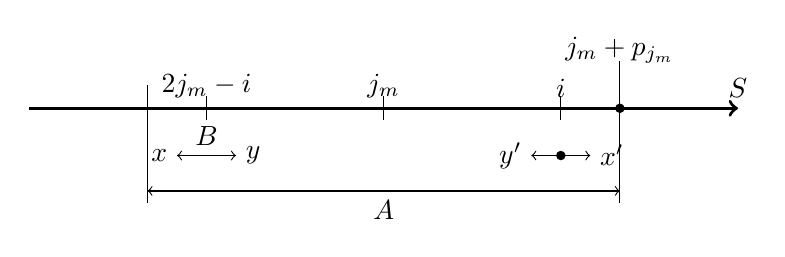
\begin{tikzpicture}[scale=1.5]
  \draw[->, very thick] (-3, .5) --(-1.5, .5) node[above]{$2j_m - i$} --
         (0, .5) node[above]{$j_m$} -- (1.5, .5) node[above]{$i$} --
         (3, .5) node[above]{$S$};
  \draw[thin] (1.5, 0.4) -- + (0, .2); %tick for i
  \draw[thin] (-1.5, 0.4) -- + (0, .2); %tick for 2j_m - i
  \draw[thin] (0, 0.4) -- + (0, .2); %tick for j_m

  % label j_m + p_{j_m}
  \draw (2, .8) node[above]{$j_m + p_{j_m}$};
  \filldraw (2, .5) circle [radius=1pt];

  % palindrome A
  \draw[<->] (-2, -0.2) -- +(2, 0) node[below]{$A$} -- (2, -0.2);
  \draw[thin] (-2, -0.3) -- +(0, 1);   %left bound for S[j_m, P_{j_m}]
  \draw[thin] (2, -0.3) -- + (0, 1.2); %right bound for S[j_m, P_{j_m}]

  % palindrome B
  \draw[<->] (-1.75, .1) node[left]{$x$} -- (-1.5, .1) node[above]{$B$} -- (-1.25, .1) node[right]{$y$};

  % palindrome at i
  \draw[<->] (1.25, .1) node[left]{$y'$} -- (1.75, .1) node[right]{$x'$};
  \filldraw (1.5, .1) circle [radius = 1 pt];

\end{tikzpicture}
\caption{$left(A) < left(B)$}
\label{fig:subcase2}
\end{figure}

This fact indicates the result of sub case 2 is $p_i = p_{2j_m - i}$.

\subsubsection*{Sub-case 3}

\begin{figure}[htdp]
\centering
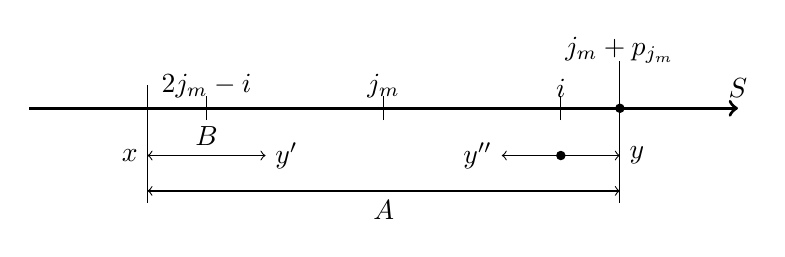
\begin{tikzpicture}[scale=1.5]
  \draw[->, very thick] (-3, .5) --(-1.5, .5) node[above]{$2j_m - i$} --
         (0, .5) node[above]{$j_m$} -- (1.5, .5) node[above]{$i$} --
         (3, .5) node[above]{$S$};
  \draw[thin] (1.5, 0.4) -- + (0, .2); %tick for i
  \draw[thin] (-1.5, 0.4) -- + (0, .2); %tick for 2j_m - i
  \draw[thin] (0, 0.4) -- + (0, .2); %tick for j_m

  % label j_m + p_{j_m}
  \draw (2, .8) node[above]{$j_m + p_{j_m}$};
  \filldraw (2, .5) circle [radius=1pt];

  % palindrome A
  \draw[<->] (-2, -0.2) -- +(2, 0) node[below]{$A$} -- (2, -0.2);
  \draw[thin] (-2, -0.3) -- +(0, 1);   %left bound for S[j_m, P_{j_m}]
  \draw[thin] (2, -0.3) -- + (0, 1.2); %right bound for S[j_m, P_{j_m}]

  % palindrome B
  \draw[<->] (-2, .1) node[left]{$x$} -- (-1.5, .1) node[above]{$B$} -- (-1, .1) node[right]{$y'$};

  % palindrome at i
  \draw[<->] (1, .1) node[left]{$y''$} -- (2, .1) node[right]{$y$};
  \filldraw (1.5, .1) circle [radius = 1 pt];

\end{tikzpicture}
\caption{$A$ and $B$ are aligned on the left.}
\label{fig:subcase2}
\end{figure}

\begin{thebibliography}{99}

\bibitem{Ukkonen95}
Esko Ukkonen. ``On-line construction of suffix trees''. Algorithmica 14 (3): 249--260. doi:10.1007/BF01206331. http://www.cs.helsinki.fi/u/ukkonen/SuffixT1withFigs.pdf

\bibitem{Manacher75}
Manacher, Glenn (1975), ``A new linear-time `on-line' algorithm for finding the smallest initial palindrome of a string'', Journal of the ACM 22 (3): 346�C351, doi:10.1145/321892.321896

\bibitem{wiki-longest-palindrome}
Longest palindromic substring. Wikipedia. http://en.wikipedia.org/wiki/Longest\_palindromic\_substring

\end{thebibliography}

\end{document}
